\chapter{Quick Start Example}\label{chap:example}

This chapter provides a brief introduction to \Kieker{} based on a simple Bookstore example application. %
Section \ref{sec:example:downloadInstall} explains how to download and install \Kieker{}. The Bookstore application itself is introduced in Section \ref{sec:example:bookstore}, while the following Sections \ref{sec:example:monitoring} and \ref{sec:example:analysis} demonstrate how to use \Kieker{} for monitoring and analyzing the resulting monitoring data.

\section{Download and Installation}\label{sec:example:downloadInstall}

\Kieker{} can be downloaded from \KiekerURL. The web site provides zip/tar.gz archives of the \Kieker{} binary distribution as well as the corresponding \Kieker{} source code archives.

For this chapter, it is required to download and extract an archive containing \Kieker's binary distribution, e.g., \file{\binaryFileForDownload}. The extracted content has roughly the following directory structure:
% Note: The indention is not really necessary, but the tree is easier to understand in the tex-source.
\begin{figure}[H]
\begin{graybox}
\dirtree{%  
	.1 \DirInDirTree{\KiekerDir/}.
		.2 \DirInDirTree{bin/}\DTcomment{Call scripts for \Kieker{} tools}. 
			.3 \ldots. 
		.2 \DirInDirTree{doc/}\DTcomment{}. 
			.3 \DirInDirTree{tutorial/}. 
				.4 userguide.pdf\DTcomment{PDF file of this document}. 
				.4 source-example/\DTcomment{Source code of the examples in this document}. 
		.2 \DirInDirTree{dist/}\DTcomment{The \Kieker{} framework libraries}. 
			.3 \analysisJar. 
			.3 \commonJar. 
			.3 \monitoringJar. 
			.3 \toolsJar. 
		.2 \DirInDirTree{lib/}\DTcomment{Libraries required by \Kieker{}}. 
			.3 \ldots. 
		.2 \DirInDirTree{META-INF/}\DTcomment{Example configuration files}. 
			.3 \ldots. 
}
\end{graybox}
\caption{Directory structure and contents of \Kieker{}'s binary distribution}
\end{figure}

\section{Bookstore Example Application}\label{sec:example:bookstore}

The Bookstore application is a small sample application resembling a simple %
bookstore where a user can search for books in an online catalog. %
Figure~\ref{fig:bookstore:classAndSequenceDiagrams} \ldots

\begin{figure}[h]\centering
\subfigure[]{\label{fig:boostore:classdiagram}%
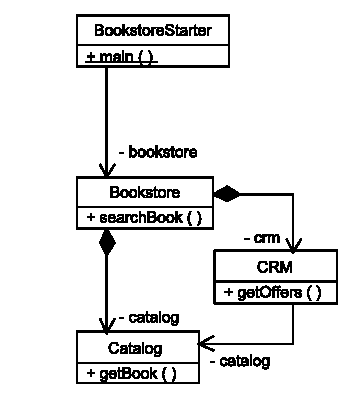
\includegraphics[scale=0.8]{images/kieker_bookstoreclassdiagram}%
}%
\subfigure[]{\label{fig:boostore:sequencediagram}%
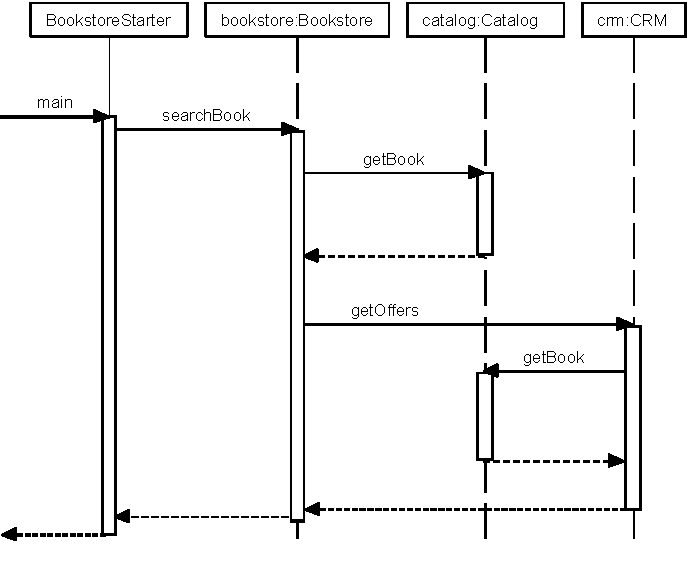
\includegraphics[scale=0.8]{images/kieker_SequenceDiagram-manually-changed}%
}
\caption{UML class diagram~\subref{fig:boostore:classdiagram} and %
sequence diagram~\subref{fig:boostore:classdiagram} of the Bookstore application}
\label{fig:bookstore:classAndSequenceDiagrams}
\end{figure}


\noindent Figure~\ref{Figure:PlainBookstoreExample} shows the directory structure of the application.

\begin{figure}[H]
\begin{graybox}
\dirtree{%
.1 \DirInDirTree{example/}. %\DTcomment{The root directory of the project}.
.2 \DirInDirTree{build/}\DTcomment{Directory for the Java class files}. 
.2 \DirInDirTree{src/}\DTcomment{The directory for the source code files}.
.3 \DirInDirTree{bookstoreApplication/}.
.4 Bookstore.java.
.4 BookstoreStarter.java.
.4 Catalog.java.
.4 CRM.java.  
}
\end{graybox}

\caption{The directory structure of the Bookstore application}
\label{Figure:PlainBookstoreExample}
\end{figure}

\noindent The following listings show the content of the source code files:

\setJavaCodeListing
\lstinputlisting[caption=Bookstore.java]{\plainBookstoreApplicationDir/src/bookstoreApplication/Bookstore.java}
\lstinputlisting[caption=CRM.java]{\plainBookstoreApplicationDir/src/bookstoreApplication/CRM.java}
\lstinputlisting[caption=Catalog.java]{\plainBookstoreApplicationDir/src/bookstoreApplication/Catalog.java}
\lstinputlisting[caption=BookstoreStarter.java]{\plainBookstoreApplicationDir/src/bookstoreApplication/BookstoreStarter.java}

\noindent The example can be compiled and executed as follows:
\setBashListing
% \begin{lstlisting}
nils@Laptop:~/example/$ javac src/mySimpleKiekerExampleManual/*.java -d build

nils@Laptop:~/example/$ java -classpath ./build/:./lib/commons-logging-1.1.1.jar\
                        mySimpleKiekerExampleManual.BookstoreMonitoringStarter 
\end{lstlisting}
% \WARNBOX{The default command-line interpreter of Windows doesn't support automatic file expansion. Therefore every single sourcefile has to be passed:
\begin{lstlisting}[caption=Commands to compile and run the Bookstore application]
#\lstshellprompt{}# javac src/bookstoreApplication/Bookstore.java 
        src/bookstoreApplication/BookstoreStarter.java 
        src/bookstoreApplication/Catalog.java 
        src/bookstoreApplication/CRM.java 
        -d build/

#\lstshellprompt{}# java -classpath build/ bookstoreApplication.BookstoreStarter 
\end{lstlisting}
%
%}

\noindent The following listing shows an example run of the application:
\begin{lstlisting}[caption=Example run of the ``plain'' application,label=lst:result-noinstr]
Bookstore.main: Starting request 0
Bookstore.main: Starting request 1
Bookstore.main: Starting request 2
Bookstore.main: Starting request 3
Bookstore.main: Starting request 4
\end{lstlisting}


\section{Monitoring}\label{sec:example:monitoring}
For the monitoring it is necessary to add some libraries from the \Kieker{}-framework to the example directory:
\begin{figure}[H]
\begin{graybox}
\dirtree{%
.1 \DirInDirTree{example/}. %\DTcomment{The root directory of the project}.
.2 \DirInDirTree{build/}\DTcomment{Directory for the Java class files}. 
.2 \newFileDirInDirTree{\DirInDirTree{lib/}}\DTcomment{Directory for the required libraries}.
.3 \newFileDirInDirTree{\monitoringJar}.
.3 \newFileDirInDirTree{\commonJar}.
.3 \newFileDirInDirTree{\commonsLoggingJar}.
.2 \DirInDirTree{src/}\DTcomment{The directory for the source code files}.
.3 \ldots.
}
\end{graybox}
\end{figure}

\noindent The \Kieker{} jar-files must be copied from the \dir{\KiekerDir/dist/} directory %
of the \Kieker{} release, as described in Section~\ref{sec:example:downloadInstall}. %
The file \file{commons-logging-1.1.1.jar} is included in \dir{\KiekerDir/lib/} %
and can also be copied from there.

The monitoring itself is done manually. Although this is not the strength of \Kieker\ it is pretty good for a quick start. Following listing shows how a method call is monitored:
\TODO{Imports?!\\ --- avh: ja, evtl. mit linerange, aber er bl\"oderweise nummeriert er so durch}
% Make sure that this listing will be modified, once the sourcecode changes!!!
% It must show the whole monitoring of the bookstorecall, from getting the first time to persisting of the record!!
\setJavaCodeListing
\lstinputlisting[linerange={11-29}, firstnumber=11, caption=Instrumentation of the \method{getBook()} call in Bookstore.java, label=listing:cuttingBookstore]%
{\manualInstrumentedBookstoreApplicationDir/src/bookstoreApplication/Bookstore.java}
 
\noindent The time before and after a specific method call (in this case: \method{searchBook()}) is remembered. These information are stored in the so called operation execution record. Its (partially) layout can be seen in Figure \ref{Figure:OperationExecutionRecordClassDiagram}.

\begin{figure}[H]
\begin{centering}
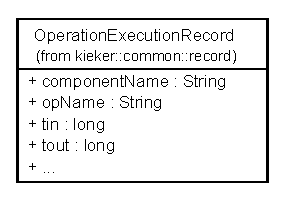
\includegraphics[scale=1]{images/kieker_OperationExecutionRecord-notraceattributes}%
\caption{The class diagram of the operation execution record}
\label{Figure:OperationExecutionRecordClassDiagram}
\end{centering}
\end{figure}

\noindent The important attributes for now are:
\begin{compactitem}
\item \class{componentName:} The component (the class) in which the called method is.
\item \class{opName:} The called method.
% \item traceId: The trace id of the current trace we want to record. Due to the fact, that we follow only one trace, this is zero in all recordings.
\item \class{tin:} The time before the source code which should be measured.
\item \class{tout:} The time after the source code which should be measured.
\end{compactitem}

\quad\\

\noindent As an example, another method in \file{CRM.java} is monitored as well:

\setJavaCodeListing
\lstinputlisting[firstline=16, firstnumber=16, lastline=27, caption=Instrumentation of the \method{getBook()} call in CRM.java, label=listing:cuttingCRM]%
{\manualInstrumentedBookstoreApplicationDir/src/bookstoreApplication/CRM.java}
The instrumented example can now be compiled and executed as follows:

\setBashListing 		
\begin{lstlisting}
nils@Laptop:~/example$ javac src/mySimpleKiekerExampleManual/*.java\
 -classpath ./lib/°\commonJar°:./lib/°\monitoringJar°:\
 -d build

nils@Laptop:~/example$ java\
-classpath ./build/:\
./lib/°\commonJar°:./lib/°\monitoringJar°:./lib/°\commonsLoggingJar°\
mySimpleKiekerExampleManual.BookstoreMonitoringStarter 
\end{lstlisting}
	

\begin{lstlisting}[caption=Commands to compile and run the instrumented Bookstore under Windows,label=lst:bookstoreStarterWin]
#\lstshellprompt{}# mkdir build
#\lstshellprompt{}# javac src\bookstoreApplication\*.java -classpath lib\#\mainJar# -d build\

#\lstshellprompt{}# java -classpath build\;
       lib\#\mainJar#;
       lib\#\commonsLoggingJar#
       bookstoreApplication.BookstoreStarter 
\end{lstlisting}


\WARNBOX{%
The default command-line interpreter of Windows doesn't support automatic %
file expansion. Therefore every single source file has to be passed, as %
shown in Listing~\ref{lst:bookstoreStarterWin}. %
Also, it is necessary to separate the different elements of the classpath with %
a semicolon instead of a colon.}

\noindent If everything worked correctly, there should now be a new directory with the %
name \dir{tpmon-20100727-181422131-UTC/} (just with another timestamp) in the default %
temporary directory (under Linux this should be \dir{/tmp/}; under Windows %
\dir{C:\textbackslash{}temp\textbackslash{}}). In this directory, there should be a file with the extension %
\dir{.dat} which contains the recorded information from the source code and %
a file named \dir{tpmon.map} which contains information about the types of the %
monitoring records. %
The Listings~\ref{listing:exampledat} and \ref{listing:examplemap} show example %
contents. 
\begin{figure}[H]
\begin{graybox}
\dirtree{%
.1 \DirInDirTree{/tmp/}.
.2 \DirInDirTree{tpmon-20100727-181422131-UTC/}.
.3 tpmon.map.
.3 tpmon-20100727-181422234-UTC-Thread-2.dat.
}
\end{graybox}
\end{figure}

\setBashListing
\lstinputlisting[caption=tpmon-20100727-181422234-UTC-Thread-2.dat (excerpt), firstline=1, lastline=3, label=listing:exampledat]%
{ch2-quickstart-example/tpmon-20100727-181422131-UTC/tpmon-20100727-181422234-UTC-Thread-2.dat}

\lstinputlisting[caption=tpmon.map, label=listing:examplemap]%
{ch2-quickstart-example/tpmon-20100727-181422131-UTC/tpmon.map}

\noindent The \file{.dat}-file is saved as a CSV-file (\textbf{C}omma \textbf{S}eparated \textbf{V}alues), meaning that it can be opened with Microsoft Excel or OpenOffice.org Calc. It would be possible to visualize the stored data with the help of these programs, but we will show in Section \ref{sec:example:analysis} how to use \KiekerAnalysisPart\ to read and process the files.

\section{Analysis}\label{sec:example:analysis}
As mentioned in the beginning of this chapter, it is shown how a simple consumer is programmed before starting the analysis. Therefore we need some new files:
\begin{figure}[H]
\begin{graybox}
\dirtree{%  
.1 \DirInDirTree{example/}. 
.2 \DirInDirTree{build/}\DTcomment{Directory for the Java class files}. 
.2 \DirInDirTree{lib/}\DTcomment{Directory for the required libraries}.
.3 \ldots. 
.3 \newFileDirInDirTree{\analysisJar}.
.2 \DirInDirTree{src/}\DTcomment{The directory for the source code files}.
.3 \DirInDirTree{bookstoreApplication/}.
.4 \ldots. 
.4 \newFileDirInDirTree{BookstoreAnalysisStarter.java}.
.4 \newFileDirInDirTree{Consumer.java}.
}
\end{graybox}
\end{figure}

\noindent The new jar-file can again be found in \dir{\KiekerDir/dist}. Listing \ref{listing:Consumer} shows the content of the new created \dir{Consumer.java}. It implements the \class{IMonitoringRecordConsumerPlugin} and overrides the necessary methods so that it can later be used by the analysis component of \Kieker. In this case the component gets a maximal response time within the constructor which will later be used to check whether a recorded method call replied fast enough or not. If the method call needed more time to response that the maximal allowed response time, it will be written directly to the error stream.\\
The methods \method{terminate} and \method{execute} don't do anything due to the fact that the consumer doesn't need any initialization. If the consumer would for example use threads then these methods would be the correct location to start and stop them.

\setJavaCodeListing       
\lstinputlisting[caption=Consumer.java, label=listing:Consumer]{\manualInstrumentedBookstoreApplicationDir/src/bookstoreApplication/Consumer.java}

\noindent Now, we have to create the file \dir{BookstoreAnalysisStarter.java} to analyze our recorded information. 

The analysis consists thereby of the following steps:
\begin{compactenum}
\item Create a new instance (or more) of the class \class{AnalysisInstance}.
\item Register the plugins which should evaluate the records.
\item Register exactly one reader to read the stored information.
\item Start the analysis instance.
\end{compactenum}

\setJavaCodeListing       
\lstinputlisting[caption=BookstoreAnalysisStarter.java]{\manualInstrumentedBookstoreApplicationDir/src/bookstoreApplication/BookstoreAnalysisStarter.java}
As can be seen, the application expects the output directory from the earlier monitoring run (see Section \ref{sec:example:monitoring}) as argument, which must be passed manually. Following listings show again the course of action:
\setBashListing 		
\begin{lstlisting}[caption=Commands to compile and run the analysis under \UnixLikeSystems{},label=lst:bookstoreAnalysisStarterLinux] 			
#\lstshellprompt{}# mkdir build
#\lstshellprompt{}# javac src/kieker/examples/userguide/ch2bookstore/manual/*.java 
        -classpath lib/#\mainJarEMF# -d build/

#\lstshellprompt{}# java -classpath build/:lib/#\mainJarEMF#
       kieker.examples.userguide.ch2bookstore.manual.BookstoreAnalysisStarter 
       /tmp/kieker-20120402-163314855-UTC-myHost-KIEKER-SINGLETON
\end{lstlisting}		
\begin{lstlisting}[caption=Commands to compile and run the analysis under Windows,label=lst:bookstoreAnalysisStarterWin]
#\lstshellprompt{}# mkdir build
#\lstshellprompt{}# javac src\kieker\examples\userguide\ch2bookstore\manual\*.java 
        -classpath lib\#\mainJarEMF# -d build\

#\lstshellprompt{}# java -classpath build\;lib\#\mainJarEMF#
       kieker.examples.userguide.ch2bookstore.manual.BookstoreAnalysisStarter 
       C:\Temp\kieker-20130910-120352847-UTC-myHost-KIEKER-SINGLETON
\end{lstlisting}	

	
It should be ensured that the application gets the correct path from the monitoring run. 

If everything worked correctly, the consumer should write something on the outputstream for every record it gets. A possible display of the run can be found in the appendix of this tutorial. 